\section{Malacology: A Programmable Storage System}
\label{sec:malacology}

\begin{table*}
\centering\small
\begin{tabular}{ l | c | l | l | l }
%\multicolumn{4}{c}{\Large \textbf{Common Internal Abstractions}} \\
\multicolumn{4}{c}{} \\
\textbf{Interface}                      &
\textbf{Section}                        &
\textbf{Example in Production Systems}  &
\textbf{Example in Ceph}                &
\textbf{Provided Functionality}            \\ \hline
Service Metadata
  & \S\ref{sec:service-metadata-interface}
  & Zookeeper/Chubby coordination~\cite{hunt_zookeeper_2010,burrows_chubby_2006}
  & cluster state management~\cite{website:ceph-mon}
  & consensus/consistency
  \\
Data I/O
  & \S\ref{sec:data-io-interface}
  & Swift in situ storage/compute~\cite{website:zerocloud}
  & object interface classes~\cite{website:cls-lua}
  & transaction/atomicity
  \\
Shared Resource
  & \S\ref{sec:shared-resource-interface}
  & MPI collective IO, burst
  & POSIX metadata protocols
  & serialization/batching
  \\
File Type
  & \S\ref{sec:file-type-interface}
  & ?????
  & file striping strategy
  & data/metadata access
  \\
Load Balancing
  & \S\ref{sec:load-balancing-interface}
  & VMWare's VM migration~\cite{vmware-drs,gulati:hotcloud2011-cloud-resource-management} 
  & migrate POSIX metadata~\cite{weil:sc2004-dyn-metadata}
  & migration/sampling
  \\
Durability
  & \S\ref{sec:durability}
  & S3/Swift interfaces (RESTful API)
  & object store library~\cite{weil_rados_2007}
  & persistence/safety
  \\
\end{tabular}
\caption{Common internal abstractions. The same ``internal abstractions" common
across large-scale systems because they provide primitives that solve general
distributed systems problems.  Here we list examples of what these internal
abstractions are used for in ``production systems" and in Ceph.  Malacology
provides these internal abstractions as interfaces
\newcomment{(Section~\ref{sec:malacology})} that higher level
\oldcomment{applications} \newcomment{services (Section~\ref{sec:services})}
can use.  \oldcomment{; {\it italicized abstractions} are interfaces discussed
in this paper.}}
\addressesissue{1}
\label{table:examples}
\end{table*}

The guiding principle is to re-use existing services and extend them so that
these services can be \emph{programmed}. We accomplish programmability of a
service by exporting bindings (or ``hooks'') for an interpreted programming
language so that programming can occur without having to restart the storage
system (see also below,~\S\ref{sec:durability}). Table~\ref{table:examples}
shows the internal services from Ceph that we expose in the Malacology
prototype via Lua~\cite{ierusalimschy1996lua} bindings\oldcomment{.}
\newcomment{and Figure~\ref{fig:implementation-overview} compares what was
already present in Ceph (gray boxes) to the Malacology interfaces we added.
Section~\ref{sec:services} will describe the higher-level services we built
with these interfaces.} \addressesissue{1}

\begin{figure}[tbp]
\centering
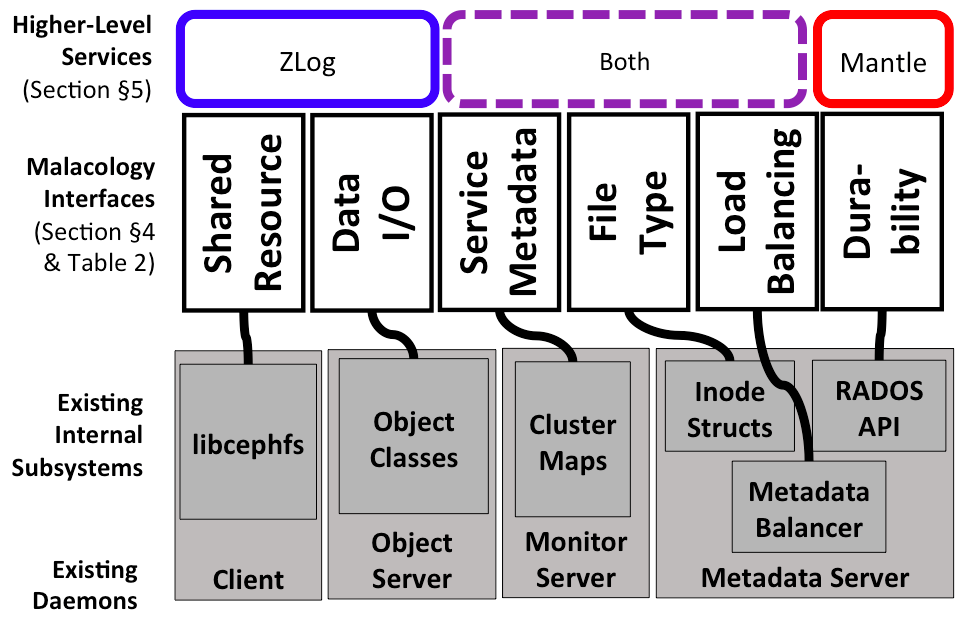
\includegraphics{figures/implementation-overview.png}
\caption{\newcomment{Malacology is implemented on the daemons and clients that
run in a Ceph cluster. Interfaces expose internal subsystems and are used as
building blocks for higher-level services.}\addressesissue{1}
\label{fig:implementation-overview}}
\end{figure}

Lua is a portable embedded scripting language and we choose it as the
interpreted language for Malacology because it offers superior performance and
productivity trade-offs, including a JIT-based implementation that is well
known for near native performance. Additionally, Lua has been used extensively
in game engines, and systems research \cite{neto:dls14-luaos}, including
storage systems where it has been effectively used both on
\cite{grawinkel:pdsw2012-lua,watkins2013:bdmc13-in-vivo,geambasu_comet_2010}
and off \cite{sevilla:sc15-mantle} the performance critical path. Finally, the
flexibility of the runtime allows execution sandboxing in order to address
security and performance concerns. We will now discuss the common subsystems
used to manage storage system and how Malacology makes them programmable.

\subsection{Service Metadata Interface}
\label{sec:mon}
\label{sec:service-metadata-interface}
\label{service-metadata}

% straw man example
Keeping track of state in a distributed system is an essential part of any
successful service and a necessary component in order to diagnose and detect
failures, when they occur. This is further complicated by variable propagation
delays and heterogeneous hardware in dynamic environments.
\newcommentone{Service metadata is information about the daemons in the system
and includes membership details, hardware layout ({\it e.g.}, racks, power
supplies, etc.), data layout, and daemon state/configuration. It differs from
traditional file system metadata which is information about files. For the rest
of the paper when we use the phrase ``metadata server" or ``metadata service",
we are referring to the daemon(s) that manages file system metadata.}
\addressesissue{4}

\newcomment{\\ \noindent\it{\textbf{Existing Ceph Implementation: }}} In the
case of Ceph, a consistent view of cluster state among server daemons and
clients is critical to provide strong consistency guarantees to clients.  Ceph
maintains cluster state information in per-subsystem  data structures called
``maps'' that record membership and status information.  A
Paxos~\cite{lamport_parttime_1998} monitoring service is responsible for
integrating state changes into cluster maps, responding to requests from
out-of-date clients and synchronizing members of the cluster whenever there is
a change in a map so that they all observe the same system state. As a
fundamental building block of many system designs, consensus abstractions such
as Paxos are a common technique for maintaining consistent data versions, and
are a useful system to expose.

The default behavior of the monitor can be seen as a Paxos-based notification
system, similar to the one introduced in~\cite{burrows_chubby_2006}, allowing
clients to identify when new values (termed epochs in Ceph) are associated to
given maps.  Since Ceph does not expose this service directly, as part of our
Malacology implementation, we expose a key-value service designed for managing
\oldcommentone{configuration} \newcommentone{service} metadata that is built on
top of the consensus engine. Since the monitor is intended to be out of the
high-performance I/O path, a general guideline is to make use of this
functionality infrequently and to assign small values to maps.\\

\noindent{\it{\textbf{Malacology: }}} Malacology exposes a strongly-consistent
view of time-varying service metadata as a service rather than a hidden
internal component. Malacology provides a generic API for adding arbitrary
values to existing subsystem cluster maps. As a consequence of this,
applications can define simple but useful service-specific logic to the
strongly-consistent interface, such as authorization control (just specific
clients can write new values) or triggering actions based on specific values
(e.g. sanitize values).  The higher-level services we implement in
\S\ref{sec:services} make use of this functionality to register, version and
propagate dynamic code (Lua scripts) for new object interfaces defined in
storage daemons (\S\ref{object-data-interface}) and policies in the load
balancer \S\ref{malacology:mds}.  Using this service guarantees that interface
definitions are not only made durable, but are transparently and consistently
propagated throughout the cluster so that clients are properly synchronized
with the latest interfaces.\\

\noindent\newcomment{{\it{\textbf{Impact: }}} provides core functionality
because it lets daemons come to consensus on system critical state. Bugs in the
internal subsystems or ommitting this from services that need this type of
consistency affects correctness.} \addressesissue{3, 5}

%And finally, it is important to not underestimate the importance of the
%preservation of the modifications that enable a new system service. In many
%(if not all) cases, interfaces defining access to data are just as important
%as the data itself by virtue of inherently providing structural context. Thus,
%all components of a system service must be kept to the same standards of
%protection as data in the system itself.

\oldcomment{\noindent 4.2 Object I/O Intefrace}
\subsection{Data I/O Interface}
\label{sec:data-io-interface}
\label{object-data-interface}

Briefly described in Section~\ref{sec:application-specifc-storage-stacks}, Ceph
supports application-specific object interfaces~\cite{weil_rados_2007}. The
ability to offload computation can reduce data movement, and transactional
interfaces can significantly simplify construction of complex storage
interfaces that require uncoordinated parallel access.

\newcomment{\\ \noindent\it{\textbf{Existing Ceph Implementation: }}} An object
interface is a plugin structured similarly to that of an RPC in which a
developer creates a named function within the cluster that clients may invoke.
In the case of Ceph each function is implicitly run within the context of an
object specified when the function is called. Developers of object interfaces
express behavior by creating a composition of native interfaces or other custom
object interfaces, and handle serialization of function input and output.  A
wide range of native interfaces are available to developers such as reading and
writing to a byte stream, controlling object snapshots and clones, and
accessing a sorted key-value database. These native interfaces may be
transactionally composed along with application specific logic to create
semantically rich interfaces. An example would be an interface that atomically
updates a matrix stored in the bytestream and an index of the matrix stored in
the key-value database.\\

\begin{figure}[tbp]
\centering
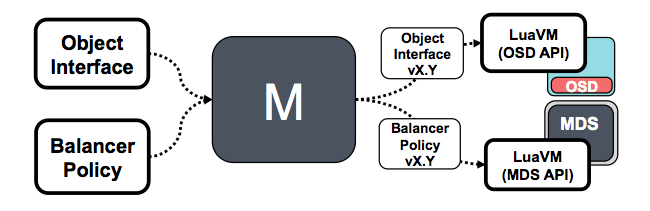
\includegraphics{figures/implementation.png}
\caption{Malacology allows users to dynamically define
object/\newcommentone{file system} metadata interfaces by extending the object
storage daemon (OSD) and metadata server (MDS) subsystems with an embedded Lua
VM.  It uses the service metadata interface (M) to propagate
interfaces/versions across the cluster \label{fig:implementation}}
\end{figure}

\noindent {\it{\textbf{Malacology: }}} The implementation of Ceph's object
abstraction, although powerful, does not readily support programmability.
Supporting only C/C++ for object interface developers, Ceph requires
distribution of compiled binaries for the correct architecture, adding a large
barrier of entry for developers and system administrators. Second, having no
way to dynamically unload modules, any changes require a full restart of a
storage daemon which may have serious performance impacts due to loss of cached
data. And finally, the security limitations of the framework limit the use of
object interfaces to all but those with administrative level access and deep
technical expertise.

To address these concerns, Malacology takes advantage of Lua extensions
contributed by the Ceph community. This allows new object interfaces to be
dynamically loaded into the system and modified at runtime, resulting in a
object storage API with economy of expression, which at the same time provides
the full set of features of the base object class. New object interfaces that
are expressed in thousands of lines of code can be implemented in approximately
an order of magnitude less code~\cite{geambasu_comet_2010}. While the use of
Lua does not prevent deployment of malicious code, certain types of coding
mistakes can be handled gracefully, and access policies are used to limit
access to trusted users~\cite{ierusalimschy1996lua}.

\oldcomment{All of these modifications work in tandem to implement the desired
behavior, and are typically co-designed together such that each depends on the
other to behave as expected.} \newcomment{\\ \noindent {\it{\textbf{Impact: }}}
helps applications optimize performance by pushing behavior to lower parts of
the storage stack, thereby minimizing hops and distributing computation.}
\addressesissue{3, 5}

\subsection{Distributed Metadata Interfaces}
\begin{notes}
\textcolor{red}{This section has been re-organized}
\end{notes}
\label{sec:distributed-metadata-interfaces}
\label{malacology:mds}

\oldcomment{The distributed metadata service in Ceph provides clients with a
POSIX file system abstraction~\cite{weil:sc2004-dyn-metadata}.}
\newcomment{File systems provide clients with the familiar POSIX file
abstraction.  While this guarantees strong consistency it comes at the cost of
scalability, increased complexity, and lower performance.} \addressesissue{1}
In general, distributed file systems protect resources by providing
hierarchical indexing and distributed locking services.  

%The metadata cluster moves units of the namespace called directory fragments
%and assigns them to servers using its own metadata load balancer. It then uses
%a hard-coded policy to balance these fragments using a scalarized load metric
%based on CPU, workload, and file system operation metrics. Although the CephFS
%balancer has been shown to be complicated, its complexity is justifiable.
%Having the flexibility to choose what to move, where to move it, and how much
%to move is very powerful. The problem is that it is difficult to pick a
%one-size-fits-all policy, system administrators may want to partition load
%based on SLAs, or applications are better equipped to make these decisions,
%etc. -- but we choose instead to expose a balancing API at strategic points in
%the balancing logic using Lua hooks. ~\cite{sevilla:sc15-mantle}. 

\oldcomment{\it{\textbf{Malacology:}} Interfaces are added in strategic spots
in the \newcommentone{file system} metadata servers for guarding shared
resources, defining new file types, and load balancing.}

\oldcomment{\noindent Shared resource interface.}
\subsubsection{Shared Resource Interface}
\label{sec:shared-resource-interface}

In general, file system metadata servers manages client sessions, allowing
clients to obtain locks (e.g. file byte ranges), and capabilities (e.g. to
cache file data). Clients and metadata servers use a cooperative protocol in
which clients voluntarily release resources back to the \newcommentone{file
system} metadata service in order to implement sharing policies.

\newcomment{\\ \noindent\it{\textbf{Existing Ceph Implementation: }}} In Ceph,
the locking service implements a capability-based system that expresses what
data and \newcommentone{file system} metadata clients are allowed to access as
well as what state they may cache and modify locally.  While designed for the
file abstraction, indexing, locking, and caching are all common services that
are useful to a broad spectrum of applications.  Distributed applications that
share centralized resources (e.g. a database or directory) face similar
challenges which are often solved using application-specific sharding.

\newcomment{\\ \noindent\it{\textbf{Malacology: }}} While the current policy
for sharing access and voluntarily releasing resources is largely best-effort,
Malacology supports generalized policies between metadata servers and clients
that can be used to implement fairness or priority.

\newcomment{\\ \noindent {\it{\textbf{Impact: }}} provides core functionality
to protect and provide exclusive access for any shared resource. May hurt
performance if the resource in question does not require strong consistency.}
\addressesissue{3}

\oldcomment{\noindent File type interface.}
\subsubsection{Malacology: File Type Interface}
\label{sec:file-type-interface}

Applications that manage large amounts of \newcommentone{file system} metadata
(e.g. users or database snapshots) often require a naming service.  The
metadata service manages a POSIX file system hierarchy where files and
directories are represented as inode data structures and expose a POSIX file
interface. 

\newcomment{\\ \noindent {\it{\textbf{Existing Ceph Implementation: }}} CephFS
is the POSIX compliant file system that uses Ceph.  Inodes are quite large (1KB
for an inode, 400 bytes for a directory entry, and 700 bytes for a directory)
and contain CephFS-specific policies like how to stripe data across RADOS.}

\newcomment{\\ \noindent {\it{\textbf{Malacology: }}}} We allow new inode types
to be defined such that applications can create domain-specific interfaces to
inodes that may modify locking and capability policies. We will show how this
is used in Section~\ref{sec:seq} when we discuss a distributed shared-log built
on Malacology.

\newcomment{\\ \noindent {\it{\textbf{Impact: }}} this interface is both a
feature and a performance optimization. It is a feature because it allows
developers to add support for different  storage types, such as how to read new
file formats or what consistency semantics to use for a specific subtree in the
hierarchical namespace. It is also a performance optimization because future
programmers can add optimizations for processing specific types of files into
the inode itself.} \addressesissue{3}

%%% TODO: striping strategy is stored with the inode

\oldcomment{\noindent \bf Load balancing interface.} 
\subsubsection{Load Balancing Interface}
\label{sec:load-balancing-interface}

\newcomment{Many large scale storage systems separate file system metadata and
data IO so that the corresponding services can scale independently. Metadata
requests transfer small amounts of data and they happen relatively frequently
so many systems employ separate file system metadata clusters.}

\newcomment{\\ \noindent {\it{\textbf{Existing Ceph Implementation: }}}} Ceph
also addresses the challenge of balancing \newcommentone{file system} metadata
load with a separate metadata cluster. This cluster uses load balancing
policies to migrate directory inodes around the cluster to alleviate overload
at single nodes~\cite{weil:sc2004-dyn-metadata}.  The policies use metrics
based on system state (e.g.  CPU and memory utilization) and statistics
collected by the cluster (e.g. the popularity of an inode). Ceph uses dynamic
subtree partitioning to move variable sized namespace subtrees. These units can
be shipped anywhere (i.e., to any metadata server of any capacity) at any time
for any reason. The original balancer was designed with hard-coded policies and
tunables.\\

\noindent {\it{\textbf{Malacology: }}} the existing load balancing mechanisms
are exposed through an API and programmers can customize the behavior through a
domain specific language. These mechanisms include the ability to migrate,
partition, and measure load. Using the Service Metadata and Durability
interfaces, this Load Balancing interface can safely version balancer policies,
save balancer policies in the back-end object store and centralize
warnings/errors. When combined with the File Type interface, load balancing
policies can express a variety of rules for handling multi-tenant and
workloads.

\newcomment{\\ \noindent {\it{\textbf{Impact: }}} helps applications optimize
performance by allowing them to specify how to partition, replicate, and
distribute metadata in response to overloaded servers.} \addressesissue{3}

\subsection{Durability Interface}
\label{sec:durability}

\newcomment{Object stores protect data using techniques like erasure coding,
replication, and data scrubbing. For scalability, many of these features are
implemented using a peer-to-peer protocol that allows object storage devices to
operate autonomously without a centralized coordinator.\\}

\noindent{\it{\textbf{Existing Ceph Implementation: }}} Ceph provides storage
by striping and replicating data across RADOS~\cite{weil_rados_2007}, the
reliable distributed object store. RADOS protects data using common techniques
such as erasure coding, replication, and scrubbing.  example, when the number
of placement groups change, the OSDs re-balance and re-shard data in the
background in a process called placement group splitting in which OSDs
communicate directly with each other to cover a new state.  In order to reduce
load on the monitoring service, Ceph OSDs use a gossip protocol to efficiently
propagate changes to cluster maps throughout the system, and autonomously
initiate recovery mechanisms when failures are discovered.\\

\noindent {\it{\textbf{Malacology: }}} Metadata service policies and object
storage interfaces are stored durability within RADOS and managed by storing
references with the object maps. Since the cluster already propagates a
consistent view of these data structures, we use this service to automatically
install interfaces in OSDs, and install policies within the metadata server
daemon (MDS) such that clients and daemons are synchronized on
correct implementations without restarting.

\newcomment{\\ \noindent {\it{\textbf{Impact: }}} this is a feature because it
adds data safety and persistence to system metadata; while nice to have it does
not necessarily effect correctness.} \addressesissue{3}
